\documentclass[12pt]{article}
\usepackage[utf8]{inputenc}
\usepackage[english]{babel}
\usepackage{amsmath}
\usepackage{amsfonts}
\usepackage{amssymb}

\usepackage[pdftex]{graphicx}
\usepackage{epsfig}
\usepackage{epstopdf}
\usepackage{multirow}

\usepackage{rotating}

%% MATH -----------------------------------------------------------
\newcommand{\modulo}[1]{\vert#1\vert}
\newcommand{\norm}[1]{\left\Vert#1\right\Vert}
\newcommand{\abs}[1]{\left\vert#1\right\vert}
\newcommand{\set}[1]{\left\{#1\right\}}
\newcommand{\Real}{\mathbb R}
\newcommand{\eps}{\varepsilon}
\newcommand{\To}{\longrightarrow}
\newcommand{\BX}{\mathbf{B}(X)}
\newcommand{\A}{\mathcal{A}}
\newcommand{\Cero}{\mathbf 0}


%% DATOS AUTORES --------------------------------------------------
\author{Pedro Diamel Marrero Fernandez \\ Juan González Hidalgo} 
\title{Projeto AM 2016-1: MVFCMddV and Multiclasification}

\begin{document}

\maketitle

%\begin{abstract}
%\end{abstract}


\section*{Introduction}

El objetivo de este trabajo es realizar la implementacion y evaluacion del metodo de clusters Multi-view relacional fuzzy c-medoids vectors clustering algorithm - MVFCMddV, asi como de la combinacion de clasificadores para la clasificacion de datos empleando multiples caracteristicas (feauters supspaces).  

\section{Methods}
En este punto se realiza una breve descripcion de los metodos y algoritmos empleados en este trabajo.

\subsection{MVFCMddV Algoritm}

\subsection{Bayes}
Aqui yo tengo que poner una bestera de bayes con la formula 

\subsection{MLP}

\subsection{SVM}



\section{Result and Discussion }


\subsection{MVFCMddV methods evaluate in synthetics data.}

Para la generacion de los datos sinteticos se empleo un generador aleatorio para datos normales multivarios y se generaron tres muestras de parametros: 

$$\mu_1 = [2, 2], \ \mu_2 = [-2, -1], \ \mu_3 = [7, -1] $$
$$\Sigma_1 = \left[ \begin{matrix}
2 & 0 \\ 
0 & 1
\end{matrix} \right], 
\Sigma_2 = \left[ \begin{matrix}
1 & 0 \\ 
0 & 1
\end{matrix} \right], 
\Sigma_2 = \left[ \begin{matrix}
1 & 0 \\ 
2 & 0
\end{matrix} \right] $$

Para generar tres señales diferentes a partir de una de ellas fueron rotados los datos en $\theta = 30$ y $\theta = 90$ grados ($X_i = R_i(\theta)*X$). Los resultados obtenidos para las tres señales se muestran en la Fig. \ref{fig:xy_sinteticos}.

\begin{figure}[h]
\centering
\includegraphics[width=4.5in]{../out/xy-sinteticos.eps}
\caption{Datos sinteticos generados.}
\label{fig:xy_sinteticos}
\end{figure}  

Para la aplicacio del metodo MVFCMddV se empleo la siguiente configuracion, $K = 3$, $m = 1.2$, $T = 10$, $\epsilon = 1e^{500}$. La Fig. \ref{fig:cluster_datos_sinteticos} muestra los resultados optenidos. En este caso se obtuvo un ARI de $0.98$.


\begin{figure}[h]
\centering
\includegraphics[width=4.5in]{../out/clusters-gauss-3.eps}
\caption{Resultados optenidos por MVFCMddV. En negro se muestran los centroides iniciales y en amarillo los centroides finales optenidos por el sistema.}
\label{fig:cluster_datos_sinteticos}
\end{figure}  


\subsection{MVFCMddV methods evaluate in real data.}

Para evaluar el metodo  MVFCMddV con datos reales fue empleada Multiple Features Data Set[XXX]. This dataset consists of features of handwritten numerals (`0'--`9') extracted from a collection of Dutch utility maps.

\begin{figure}[h]
\centering
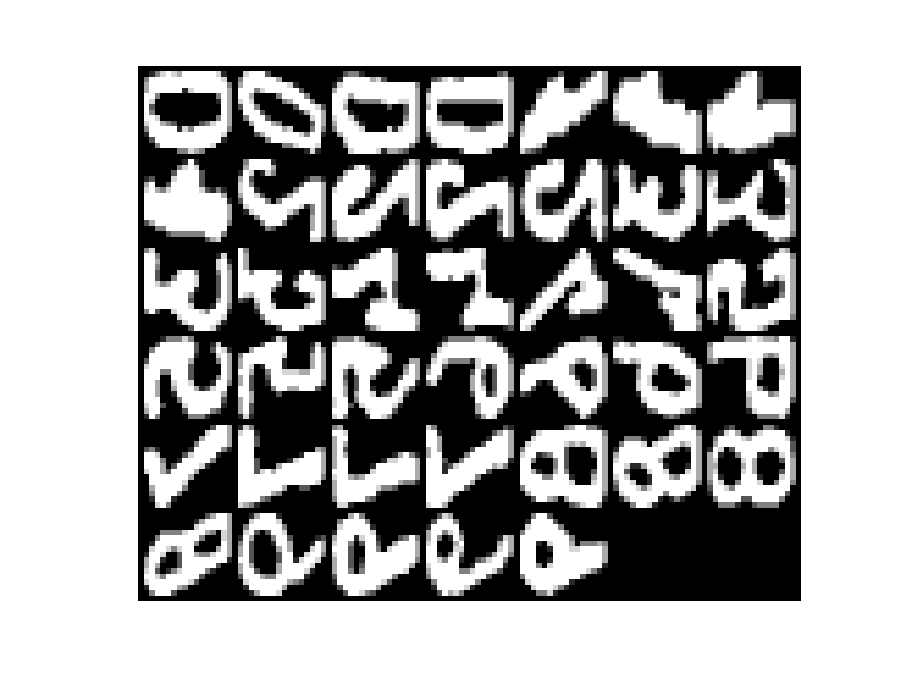
\includegraphics[width=3.5in]{../out/data-base.eps}
\caption{Multiple Features Data Set.}
\label{fig:data_base}
\end{figure}  

This dataset consists of features of handwritten numerals (`0'--`9') extracted from a collection of Dutch utility maps. 200 patterns per class (for a total of 2,000 patterns) have been digitized in binary images. These digits are represented in terms of the following six feature sets (files): (1) mfeat-fou: 76 Fourier coefficients of the character shapes; (2) mfeat-fac: 216 profile correlations; (3) mfeat-kar: 64 Karhunen-Love coefficients; (4) mfeat-pix: 240 pixel averages in 2 x 3 windows; (5) mfeat-zer: 47 Zernike moments; (6) mfeat-mor: 6 morphological features. In each file the 2000 patterns are stored in ASCI on 2000 lines. The first 200 patterns are of class `0', followed by sets of 200 patterns for each of the classes `1' - `9'. Corresponding patterns in different feature sets (files) correspond to the same original character. The source image dataset is lost. Using the pixel-dataset (mfeat-pix) sampled versions of the original images may be obtained (15 x 16 pixels).

Se selecciono para hacer los experimentos los subespacios de caracteristicas determinados por mfeat-fou, mfeat-kar y mfeat-zer. Fue executado 100 veses o algoritmo MVFCMddV simultaneamente para las 3 matrizes de dissimilaridade correspondientes a cada subspacio. En este caso se empleo la siguiente configuracion: $K =103$, $m = 1.6$, $T = 150$, $\epsilon = 1e^{10}$.


[Resultado ...]


\subsection{MVFCMddV methods in compress image problems.}

In a straightforward 24-bit color representation of an image, each pixel is represented as three 8-bit unsigned integers (ranging from 0 to 255) that specify the red, green and blue intensity values. This encoding is often refered to as the RGB encoding. Existen otros espacios de representacion del color como el CIELAB, HSB CMYK. El objetivo de este esperimento es valorar la reducion del numero de colores en el espacio RGB empleando ademas el espacio CIELAB. Una hipotesis valida es que la informacion de este nuevo espacio puede cotribuir a la creacion de clusters mas conveniente en este tipo de problemas.  

Como se puede obsevar en la Fig. \ref{fig:image_compress} se obtiene una buena aproximacion de la imagen original. Esta nueva imagen puede ser representada como 4-bits por pixel mas un diccionario de $16x24$. The original image required 24 bits for each one of the $64X64$ pixel locations, resulting in total size of $64x64x24 = 98.304$ bits. The new representation requires some overhead storage in form of a dictionary of 16 colors, each of which require 24 bits, but the image itself then only requires 4 bits per pixel location. The final number of bits used is therefore $16x24 + 64x64x4 = 16.384$ bits, which corresponds to compressing the original image by about a factor of 6.


\begin{figure}[h]
\centering
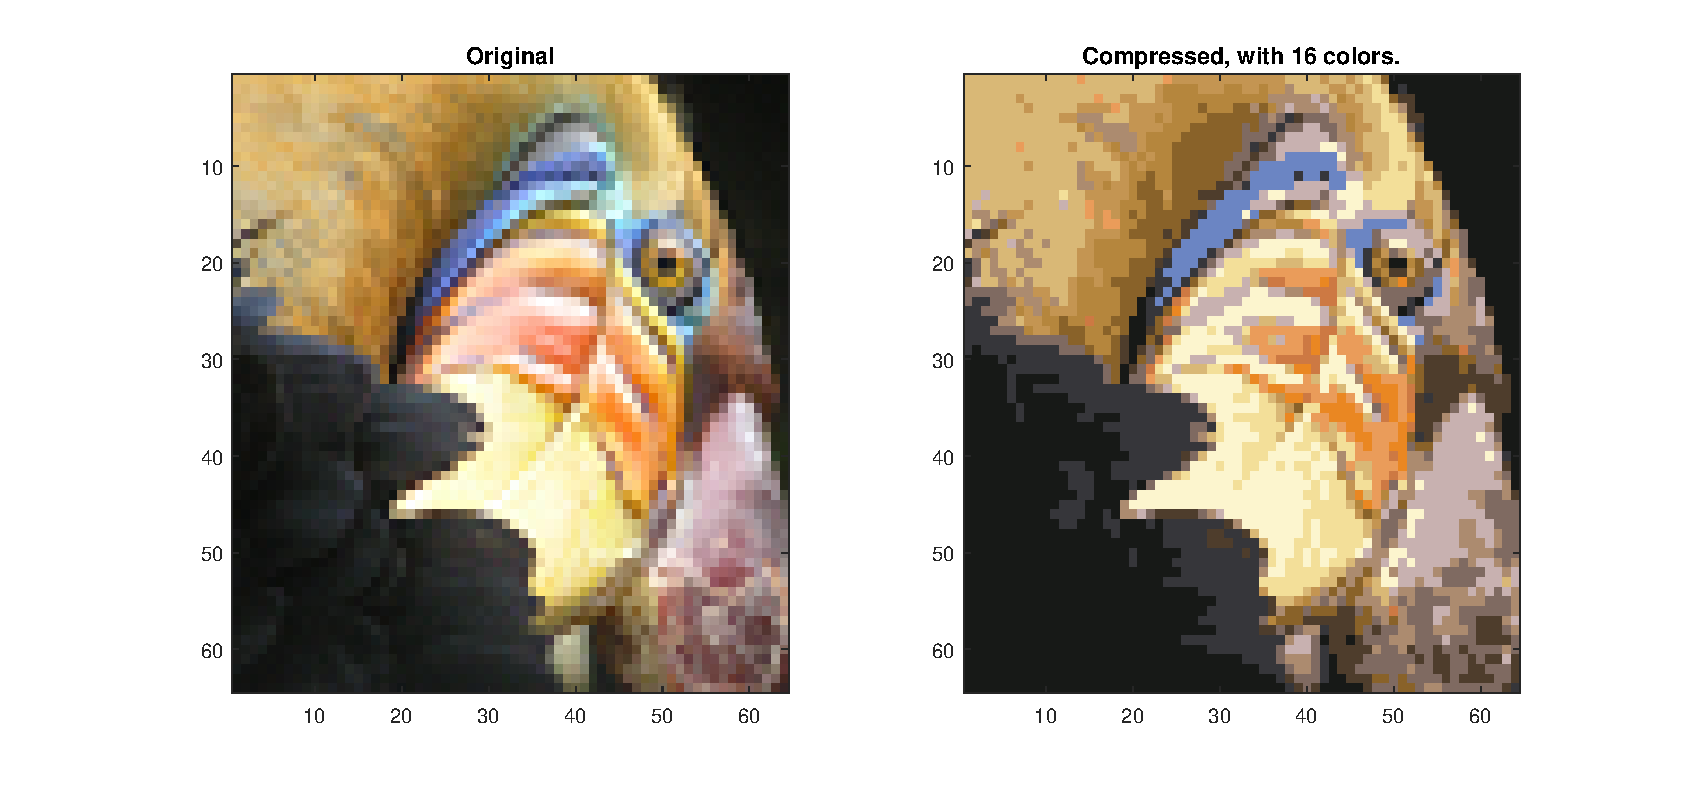
\includegraphics[width=5.5in]{../out/image-compress-16.eps}
\caption{Original and reconstructed image (when using MVFCMddV to compress the image).}
\label{fig:image_compress}
\end{figure}  


\subsection{Multiclasifcador system for multiples signal}

Para este caso tambien fue empleada la base de datos Multiple Features Data Set. 


\end{document}